% ===================================================================
% LaTeX 作业主文件 (最终优化版)
% ===================================================================

\documentclass[12pt, a4paper, twoside]{ctexart}

\usepackage{zju-homework-style-v2}
\usepackage{upgreek}
\usepackage{float}
\graphicspath{{figures/}}

\begin{document}

% --- 扉页 ---
\begin{titlepage}
    \maketitlepage
\end{titlepage}
\clearpage

% --- 作业正文 ---

% ==================== QUESTION 1 ====================
\begin{problem}
    \heiti\zihao{4}{\textcolor{QuestionBlue}{Question 1.}} Search for relevant materials to explore the knowledge of the sinc function (or Sa function) (300 - 500 words). For example, you may introduce its mathematical background and history, key properties, and connections with the development of other disciplines. In addition, identify at least two different engineering application areas (such as communications, audio processing, or image processing) and explain its role in practical problems.
\end{problem}

\vspace{5pt} % <-- 修改处:为保持一致,在此处添加间距
\subsection*{\heiti\zihao{4}Solution}
The sinc function is a fundamental mathematical function, typically defined in two forms: the \textbf{Unnormalized form},
\begin{equation*}
    \text{sinc}(x) = \frac{\sin x}{x}, \quad x \neq 0, \quad \text{sinc}(0)=1
\end{equation*}
and the \textbf{Normalized form},
\begin{equation*}
    \text{sinc}(x) = \frac{\sin(\piup x)}{\piup x}, \quad x \neq 0, \quad \text{sinc}(0)=1
\end{equation*}
The term "sinc" is derived from the Latin \textit{sinus cardinalis} (cardinal sine) and was introduced into mathematical and engineering literature by Philip M. Woodward and I. L. Davies in 1952. The function possesses several key properties that make it crucial in signal processing and communication theory. As an \textbf{Even Function}, it is symmetric about the origin, i.e., $\text{sinc}(x) = \text{sinc}(-x)$. Regarding its \textbf{Zero Crossings}, the unnormalized form is zero at non-zero integer multiples of $\piup$, while the normalized form is zero at all non-zero integers. Its \textbf{Integral Properties} are also notable: the integral of the unnormalized sinc function over the entire real line is $\piup$, whereas the integral of the normalized form is 1. Lastly, its \textbf{Fourier Transform Relationship} is fundamental; the sinc function is the Fourier transform of the rectangular function, and conversely.

In practical engineering, the sinc function has wide-ranging applications. Within \textbf{Communication Systems}, it is essential for signal reconstruction. According to the Nyquist sampling theorem, a band-limited signal can be perfectly reconstructed from its discrete samples, and the sinc function serves as the ideal interpolation kernel for this process. In \textbf{Audio Processing}, the function is used in filter design, as the impulse response of an ideal low-pass filter is a sinc function, allowing for effective preservation of low-frequency signals while suppressing high-frequency noise. Similarly, in \textbf{Image Processing}, the sinc function is employed in resampling algorithms like the Lanczos method to interpolate pixel values, which maintains high image quality during scaling or rotation.

In conclusion, due to these unique properties, the sinc function has become a fundamental tool across signal processing, communications, and image processing. It is not only an ideal interpolation kernel but also a crucial mathematical basis for filter design, making a solid understanding of it essential for engineers designing high-precision systems.

% ==================== QUESTION 2 ====================
\vspace{50pt}
\begin{problem}
    \heiti\zihao{4}{\textcolor{QuestionBlue}{Question 2.}} Use MATLAB to visualize the sinc function (or Sa function). You are required to write a program and generate a plot, mark special points in the figure (such as the maximum value and zero points), and submit both the program code and the resulting graph.
\end{problem}

\vspace{5pt} % <-- 修改处:为保持一致,在此处添加相同的间距
\subsection*{\heiti\zihao{4}Solution}

\subsubsection*{\heiti\zihao{-4}Resulting Graph}
The sinc function graph generated after executing the code is shown in Figure \ref{fig:sinc}. The plot clearly shows that the function reaches its maximum value of 1 at $t=0$ and has zero crossings at non-zero integer points.

\begin{figure}[H]
    \centering
    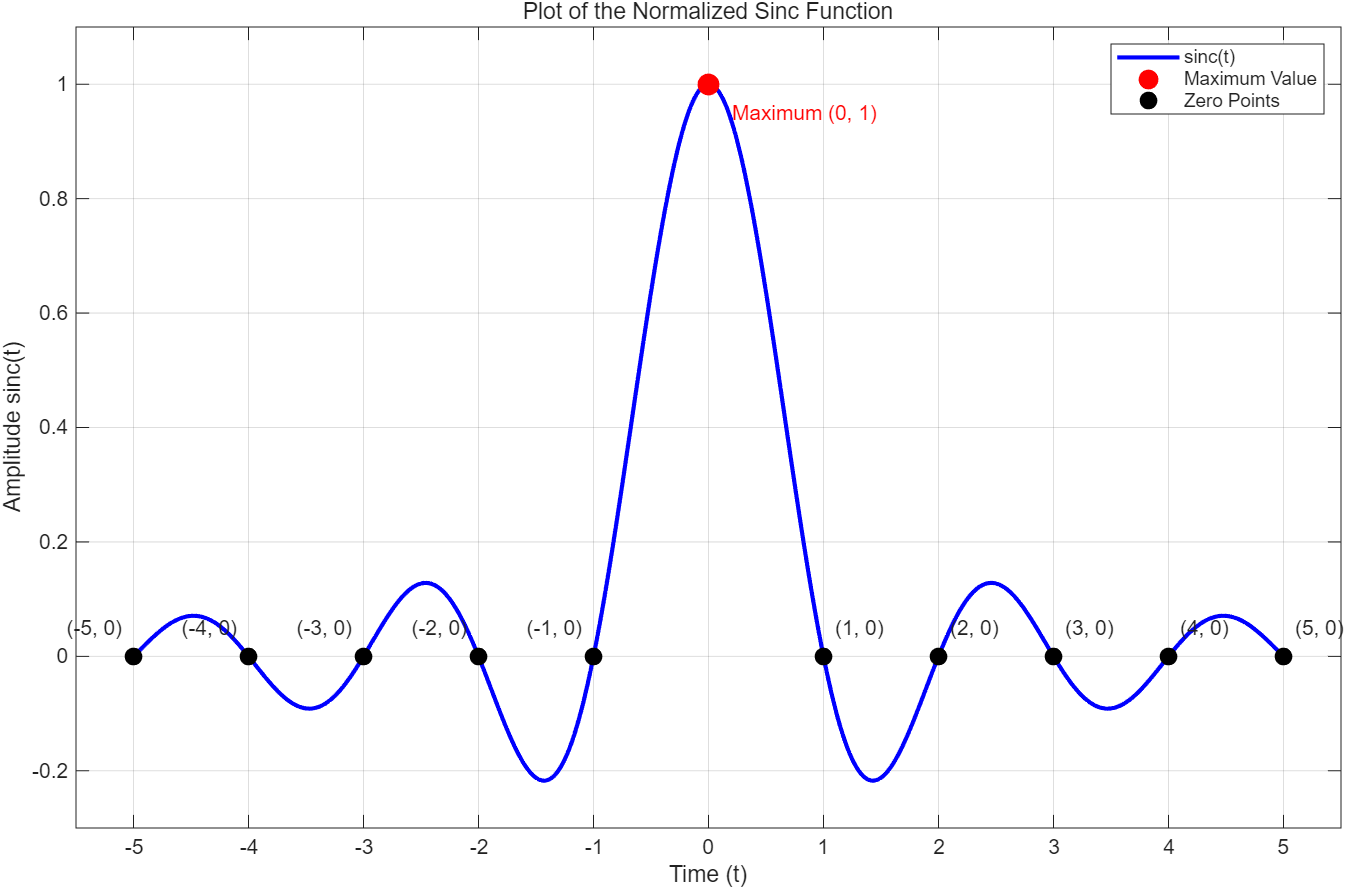
\includegraphics[width=0.85\textwidth,keepaspectratio]{sinc.png}
    \caption{Visualization of the normalized sinc function with key points marked.}
    \label{fig:sinc}
\end{figure}

\subsubsection*{\heiti\zihao{-4}Program Code}
The following is the MATLAB code used to generate the plot in Figure \ref{fig:sinc}. The code first defines a time vector, then calculates the values of the sinc function, and finally plots the graph with special points marked.

\begin{lstlisting}[style=matlabstyle, caption={MATLAB code for generating the sinc function plot.}, label={lst:sinc}]
% --- 1. Setup the Time Vector ---
t = linspace(-5, 5, 1000);

% --- 2. Calculate the Sinc Function Manually ---
y = ones(size(t)); 
t_non_zero = (t ~= 0); 
y(t_non_zero) = sin(pi * t(t_non_zero)) ./ (pi * t(t_non_zero));

% --- 3. Create the Plot ---
figure; 
plot(t, y, 'b-', 'LineWidth', 2); 
hold on; 

% --- 4. Mark Special Points ---
% Mark the maximum value
plot(0, 1, 'ro', 'MarkerSize', 10, 'MarkerFaceColor', 'r');
text(0.2, 0.95, 'Maximum (0, 1)', 'FontSize', 10, 'Color', 'r');

% Define the zero points
zero_points = -5:5; 
zero_points(zero_points == 0) = []; 

% Mark zero points with solid black dots
plot(zero_points, zeros(size(zero_points)), 'ko', 'MarkerSize', 8, 'MarkerFaceColor', 'k');

% Add text labels for each zero point using a loop
for i = 1:length(zero_points)
    zp = zero_points(i);
    label = sprintf('(%d, 0)', zp);
    
    % Adjust text alignment to prevent overlap
    if zp > 0
        text(zp + 0.1, 0.05, label, 'HorizontalAlignment', 'left');
    else
        text(zp - 0.1, 0.05, label, 'HorizontalAlignment', 'right');
    end
end

% --- 5. Finalize the Graph ---
title('Plot of the Normalized Sinc Function');
xlabel('Time (t)');
ylabel('Amplitude sinc(t)');
grid on;
axis([-5.5 5.5 -0.3 1.1]); % Slightly widened the x-axis for labels
legend('sinc(t)', 'Maximum Value', 'Zero Points');
hold off;

disp('Plot generated successfully.');
\end{lstlisting}

\end{document}